\chapter{The Solution}

I will discuss the design and implementation of each of the main components of the project separately.

\section{\tsPEG{}}

\subsection{High Level Design}

\tsPEG{} was built using TypeScript and the NodeJS JavaScript runtime. The NodeJS runtime allows us to execute JavaScript (and hence TypeScript) code locally.

The source code is hosted online at
\href{https://github.com/EoinDavey/tsPEG}{github.com/EoinDavey/tsPEG}, and the \tsPEG{} package is available on the NPM package repository at \href{https://www.npmjs.com/package/tspeg}{npmjs.com/package/tspeg}.

\tsPEG{} is self-hosting, meaning that the input parser for \tsPEG{} was generated by \tsPEG{}. The software architecture of \tsPEG{} is given in Figure~\ref{tspegdiagram}. The usage flow of using \tsPEG{} is as follows. First, the user creates a grammar file, specifying the input grammar they want to generate a parser for. The syntax for the grammar file follows a similar pattern to the familiar EBNF syntax for grammar specification. In this file, they specify the syntax rules, as well as names of AST fields, and computed properties. The \tsPEG{} binary is then called and it is passed in the grammar file.

\begin{figure}
    \caption{\tsPEG{} High Level Design}
    \label{tspegdiagram}
    \begin{center}
    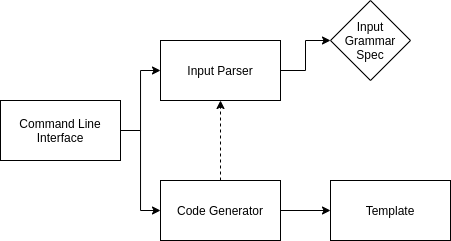
\includegraphics[scale=0.75]{tspegdiagram}
    \end{center}
\end{figure}

\tsPEG{}'s parser consumes the grammar file and generates an internal description of the grammar. The code generator then takes this grammar specification and generates parsing functions for each rule, as well as TypeScript type declarations and classes for each of the AST nodes. These functions and types are then packaged up into a template file and then written to disk.

\subsection{Grammar specification}

\tsPEG{} uses a custom syntax to define grammars. Figure~\ref{tspegexample} contains an example of a grammar specification for simple arithmetic expressions like "1+2*3".

\begin{figure}
    \caption{\tsPEG{} input grammar example}
    \label{tspegexample}
    \begin{lstlisting}[language=tspeg]
SUM  := head=FAC tail={ op='\+|-' sm=FAC }*
FAC  := head=ATOM tail={ op='\*|/' sm=ATOM }*
ATOM := val=INT
      | '\(' val=SUM '\)'
INT  := val='[0-9]+'
    \end{lstlisting}
\end{figure}

Grammars are defined by a sequence of grammar rules, for example,
    \[\texttt{match} := \texttt{rule1} \mathbin{|} \texttt{rule2} \mathbin{|} \texttt{\textquotesingle a+\textquotesingle}\]
defines a new rule called \verb|match|. \tsPEG{}'s parser will first try to match \verb|rule1|. If this match was not successful then it will try to match \verb|rule2|. Finally, if both of those matches failed, then it will try to match the regex expression \verb|a+|. If it can't match \verb|a+| then \verb|match| is considered to have failed.
    The \tsPEG{} grammar also allows specification of computed properties, for example, Figure~\ref{tspegcomputed} defines a rule to match integer literals that stores the value of the integer as a computed property.

   \textbf{Please see \hyperref[tspegdocs]{Appendix \ref*{tspegdocs}} for full documentation of \tsPEG{}'s grammar, operators and features.} 
\begin{figure}
    \caption{\tsPEG{} computed properties example}
    \label{tspegcomputed}
    \begin{lstlisting}[language=tspeg]
INT := literal='[0-9]+'
       .value = number { return parseInt(this.literal) }
    \end{lstlisting}
\end{figure}

\subsection{Bootstrapping}

When developing \tsPEG{}, first a simple input parser was written by hand, supporting only the most basic syntax. A code generator was written that could take in the AST from this simple grammar and output a parser for it. This first version acts as the foundation from which \tsPEG{} was bootstrapped. It had no extra operators, only the very foundational capabilities to define simple PEG grammars.

The meta-grammar for the input grammar syntax was subsequently written in this basic syntax. The parser generator was then ran on this grammar, this replaced the handwritten parser with a new generated one, self-hosting itself and opening itself up to bootstrapping. An interesting property of this process is that the original hand-written parser was destroyed, yet the project only functions because it did exist at some point in the past.

This new self-hosting generator was then used to add more and more features and operators to itself, eventually resulting in the full self-describing meta-grammar for the \tsPEG{} input syntax in Figure~\ref{tspegsyntax}.

\begin{figure}
    \caption{\tsPEG{} meta-grammar definition}
    \label{tspegsyntax}
    \begin{lstlisting}[language=tspeg]
GRAM      := header=HDR? rules=RULEDEF+
HDR       := '---' content='((?!---)(.|\n))*' '---'
RULEDEF   := _ name=NAME _ ':=' _ rule=RULE _
RULE      := head=ALT tail={_ '\|' _ alt=ALT }*
          .list = ALT[] { return [this.head, ...this.tail.map((x) => x.alt)]; }
ALT       := matches=MATCHSPEC+ attrs=ATTR*
MATCHSPEC := _ named={name=NAME _ '=' _}? rule=POSTOP _
POSTOP    := pre=PREOP op='\+|\*|\?'?
            .optional = boolean { return this.op !== null && this.op === '?'}
PREOP     := op='\&|!'? at=ATOM
ATOM      := name=NAME !'\s*:='
           | match=STRLIT
           | '{' _ sub=RULE _ '}'
ATTR      := _ '.' name=NAME _ '=' _ type='[^\s\{]+' _ '\{'
    action='([^\{\}\\]|(\\.))*'
'\}'
NAME      := '[a-zA-Z_]+'
STRLIT    := '\'' val='([^\'\\]|(\\.))*' '\''
_         := '\s*'
    \end{lstlisting}
\end{figure}

\subsection{Syntax Error reporting}

The parsers generated by \tsPEG{} must be capable of accurately reporting syntax errors in input strings. To achieve this an error reporting technique known as ``farthest failure'' is used. This approach is based on the approach outlined in the paper ``Error handling in PEG Parsers''\cite{pegerrors}. The idea is that the PEG parser should descend as far as possible into the input string while maintaining a valid AST, and report a syntax error at the farthest point reached in the string.

\tsPEG{} uses this approach to generated and return \verb|SyntaxError| objects. These objects contain the exact position (line and character) of the error, as well as a full list of possible symbols that could have been in that position that would have allowed the parser to continue.

\section{\Setanta{}} \label{setantasolution}

\subsection{High Level Design}
\Setanta{} is also written in TypeScript. The code structure of \Setanta{} allows it to be run as a local REPL through the NodeJS engine, but also in the browser. A high-level architecture diagram is given in Figure~\ref{setantadiagram}. The high level structure of the \Setanta{} interpreter was inspired by the high level structure of the Java tree walk interpreter of the ``Lox'' PL outlined in the book ``Crafting Interpreters''\cite{crafting-interpreters}, adapted to the needs of this project.

The \Setanta{} runtime uses the \tsPEG{} parser generator to generate its parser. Both the browser and CLI execution environments import the same interpreter and parser but provide their own set of built-in functions. Each runtime environment passes some input text to the parser, the parser returns an AST or a syntax error object. This AST can then be passed to the interpreter with the relevant builtins. The interpreter can then be stopped and started asynchronously from the main executing thread.

\begin{figure}
    \caption{\Setanta{} High Level Design}
    \label{setantadiagram}
    \begin{center}
    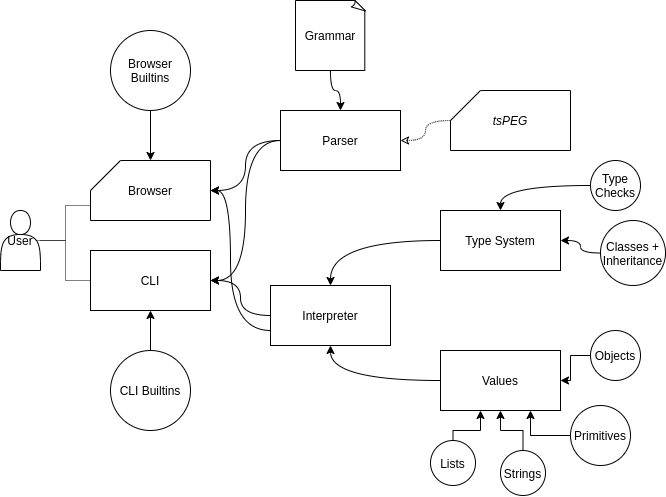
\includegraphics[scale=0.5]{setantadiagram}
    \end{center}
\end{figure}

\subsection{Syntax}

The syntax of \Setanta{} is new but should feel familiar to most people. It has been designed to be simple and approachable.

\Setanta{} programs, like most imperative languages, consist of a sequence of statements. Some important \Setanta{} features are outlined below:
\begin{itemize}
    \item \textbf{Variable declarations}

        In \Setanta{}, variables are declared using the \verb|:=| operator and can be re-assigned using the classic \verb|=| operator. The distinction is to provide a clear lexical difference between variable declaration and reassignment.
    \item \textbf{Loops + Conditionals}

        \Setanta{} supports the classic conditional execution structure of ``if, else if, else''. This is mostly a direct translation into Irish. However, it should be noted that no bracketing is required around the expression.

            \begin{lstlisting}[language=setanta, frame=single, caption=Setanta conditionals]
má x == 0
    scríobh('Tá x cothrom le 0')
nó má x == 1
    scríobh('Tá x cothrom le 1')
nó
    scríobh('Tá x níos mo ná 1')
            \end{lstlisting}

            \Setanta{} supports two main types of loops, ``le idir'' loops that allow the user to specify the start and end of the loop, and ``nuair-a'' loops, which are the familiar while loops.

            \begin{lstlisting}[language=setanta, frame=single, caption=Setanta loops]
i := 0
le i idir (0, 10)
    i = i + 1
x := 0
nuair-a x < 10
    x = x + 1
            \end{lstlisting}
        \item \textbf{Classes + Functions}

            \Setanta{} supports declaring new classes, with methods, as well as functions on their own.
            \begin{lstlisting}[language=setanta, frame=single, caption=Setanta classes]
creatlach Person ó Animal {
    gníomh nua(name) {
        name@seo = name
    }
    gníomh speak() {
        scríobh('Hi, My name is ' + name@seo)
    }
}
            \end{lstlisting}
        \item \textbf{Literals}

            \Setanta{} supports literals for integers, booleans, null, strings and lists.
            \begin{lstlisting}[language=setanta, frame=single, caption=Setanta literals]
a := 500
b := 'Dia duit domhan'
c := [1,2,3,4, fíor]
d := fíor != breag
c := neamhní
            \end{lstlisting}

\end{itemize}
            \noindent\textbf{Please see \hyperref[setantadocs]{Appendix \ref*{setantadocs}} for a full description of the syntax and semantics of \Setanta{}. The 20 page limit on the report means the full description cannot be directly included.}

\subsection{The @ operator}\label{atoperator}

One of the most important features of \Setanta{}'s syntax is the @ operator. The @ operator is where the influence of the Irish language on the design of \Setanta{} is felt most clearly. In fact, the @ operator is a simple innovation that addresses 2 distinct differences between Irish and English.

The @ operator is the lookup operator, it is used to reference member fields and methods of objects. It is functionally equivalent to the classic dot ('.') operator in C, C++, Java, Python, JavaScript etc. The subtle difference is the order, both the @ operator and the '.' operator are binary operators, but the @ operator flips its arguments compared to the '.' operator.

In the standard usage of the dot operator, the expression \verb|a.b| refers to the member ``b'' of the object ``a''. In \Setanta{} \verb|a@b| refers to the member ``a'' of the object ``b'', the order has been reversed.

This change seems unimportant, however, it breaks 2 deep and subtle links between English and the standard way we look at OOP programming languages.

Firstly, as \hyperref[background:vsosvo]{discussed in the technical background}, English is an SVO language, meaning that in English sentences, the subject comes first, then the verb, then the object. This property of English is directly reflected in the design of the classic dot operator.

The usage of the dot operator for member lookup gives rise to expressions like \verb|man.goTo(shop)|, or \verb|dbClient.query(q)|, these expressions implicitly put the subject first, then the verb, then the object, directly mimicking the SVO structure of the host language.

By using the @ operator in \Setanta{} we instead get expressions like \verb|goTo@man(shop)| or\\
\verb|query@dbClient(q)|, these expressions put the verb first, then the subject, then the object, reflecting the VSO structure of Irish. This subtle connection between a simple operator like '.' and the linguistic properties of English is not apparent at first glance.

There is a second connection between English and the lookup operation that is broken by the @ operator. In English when talking about possession relationships (``has-a'' relationships in database terms), we list the entities in decreasing order of possession, e.g.,
\begin{quote}
    The man's car door window pane
\end{quote}
The order of possession here is
\[man \rightarrow car \rightarrow door \rightarrow window \rightarrow pane\]

In direct contrast to this, in Irish we list possession in increasing order, meaning we start at the bottom of the possession relationship and work our way up. We would instead list
\[pane \leftarrow window \leftarrow door \leftarrow car \leftarrow man\]

This linguistic difference between Irish and English is again addressed by the @ operator. The standard '.' operator reflects the English language structure, \verb|man.car.door.window.pane|, but in \Setanta{}, we use the Irish ordering \verb|pane@window@door@car@man|. This is another connection between English and the standard design of PLs that is easily overlooked.

\subsection{Semantics}

The semantics of \Setanta{} will be familiar to most users, it's an imperative, strongly dynamically typed language. \Setanta{} supports a gauntlet of modern features including first-class functions, inheritance, event-based concurrency, and automatic memory management. Although \Setanta{} is an imperative language, it does support a more functional style of programming as well.

        \noindent\textbf{Please see \hyperref[setantadocs]{Appendix \ref*{setantadocs}} for a full description of the syntax and semantics of \Setanta{}.}

\subsection{Blocking operations \& Concurrency}

As discussed in the technical background section, the JavaScript runtime, whether it be NodeJS or a browser, only allows usage of a single thread and no blocking operations.
However, \Setanta{} allows the user to write and use blocking functions. Figure~\ref{blockingcomparison} shows a side by side comparison of equivalent programs in JavaScript and Setanta, it's clear that the Setanta program is much simpler due to allowing the program to block.

\begin{figure}[ht]
    \begin{minipage}[t]{0.45\textwidth}
        \begin{lstlisting}[language=javascript, caption=JavaScript]
setTimeout(() => {
    console.log('sleep1');
    setTimeout(() => {
        console.log('sleep2');
        setTimeout(() => {
            console.log('sleep3')
        }, 100);
    }, 100);
}, 100);
        \end{lstlisting}
    \end{minipage}\qquad
    \begin{minipage}[t]{0.45\textwidth}
        \begin{lstlisting}[language=setanta, caption=Setanta]
coladh(100)
scríobh('sleep1')
coladh(100)
scríobh('sleep2')
coladh(100)
scríobh('sleep3')
        \end{lstlisting}
    \end{minipage}
    \caption{Equivalent code in JavaScript + Setanta}
    \label{blockingcomparison}
\end{figure}

If you open the JavaScript console on any browser and enter \lstinline[language=javascript]|while(true){}| the browser tab will cease to be functional, i.e no buttons or text-boxes or animations will work anymore.
This is because the JavaScript engine is single-threaded, the thread is busy computing \lstinline[language=javascript]|while(true){}| and cannot process any other events.

In contrast, if you write \lstinline[language=setanta]|nuair-a fíor {}| in \Setanta{}, the browser tab will remain responsive. This is due to the implicit concurrency of all \Setanta{} functions. \Setanta{} manipulates the JavaScript engine task queue to ensure that execution time is shared between the main browser thread actions and executing the \Setanta{} code.

\subsubsection{How this was achieved}

As discussed in the \hyperref[background:asyncawait]{technical background}, Recent versions of JavaScript include a technology known as ``Promises''. These values are stand-ins for future values that are yet unknown. The \verb|Interpreter| class in \Setanta{} makes heavy use of Promises, to allow the execution of the program to be suspended at any moment. By allowing suspension of the interpreter, we allow the code to appear to block, while under the hood, the thread has not technically blocked.

This idea works in theory, but in practice, an interesting problem was observed. As outlined in the technical background, JavaScript engines use \hyperref[background:task-queues]{task queues} in the runtime to manage callbacks. Promises use this task queue to enqueue the operations that should be performed on the unknown values that they are a proxy for. However, unlike other task queue APIs exposed to the JavaScript runtime, Promises use something called the ``microtask queue''. The normal task queue is referred to then as the ``macrotask queue''. This distinction is little known, as it is usually of very little importance. However, the difference is crucial to \Setanta{}'s implementation.

When the JavaScript runtime is deciding what task to execute next, it always chooses a task from the microtask queue over any macrotask. This is because Promises are usually used to enqueue smaller operations on data, such as printing the results of web requests. However, when Promises have been used to construct a Turing complete language like \Setanta{}, we encounter the problem that while the program is running, it keeps the microtask queue full, never allowing a macrotask to be run. 

Macrotasks are important to the JavaScript runtime, and the browser especially, things like animations, scrolling, rendering, keyboard events, button presses etc. are all macrotasks. Therefore if we are blocking the macrotask queue from being executed for some long amount of time, we are preventing all these important operations from happening.

I experimented with forcing all the Promises to use the macrotask queue, rather than the microtask queue. But it turns out, the microtask queue is much faster than the macrotask queue, so this resulted in massive slowdowns. A happy medium had to be found.
My eventual solution was to allow some finite amount of microtasks to be used before a macrotask should be used instead. After experimentation on a few platforms, I found a nice number to be around 5000. Meaning that after every 5000 operations performed by the \Setanta{} runtime, it enqueues the next operation on the macrotask queue, allowing other macrotasks to be processed before the execution continues.

\subsection{Tree Compression for performance}
\label{solution:treecompression}

The arithmetic expressions in \Setanta{} have a certain operator precedence, this precedence matches the usual order of operations that we are used to. For example in the expression \verb|1 + 2 * 3|, the multiplication is performed before the addition, giving the correct answer of 7.

The grammar for \Setanta{} is carefully designed to ensure that all precedences are correct.
It's not just multiplication and addition, there are 10 different levels of precedence in the grammar for \Setanta{}.
You can see the \Setanta{} grammar spec (that \tsPEG{} uses to generate the parser) in \hyperref[appendix:setantagrammar]{Appendix \ref*{appendix:setantagrammar}}.

A side effect of this many-layered grammar specification means that simple expressions like\\
\verb|1 + 2 * 3| generate very tall, but sparse syntax trees. In Figure~\ref{setanta:uncompressedtree} you can see the full syntax tree generated for \verb|1+2*3|.
Most of these AST nodes contain no information. But in evaluating this expression directly we must traverse the entire tree.

If the expression includes variables e.g., ``\verb|a + b * c|'' we must do this every single time we evaluate it, we can't cache the result.

The solution that I came up with is to take advantage of \tsPEG{}'s \hyperref[computed-properties]{computed properties} support. Notably, this tree compression problem is exactly the problem I added computed properties to \tsPEG{} to allow me to solve.

The idea is that, at parse time, each node computes a ``shortcut'' attribute. If the node detects that it is not required, it computes a pointer to the next ``important'' node below it and returns that, shortcutting the node entirely, while maintaining the strong typing of the AST. This is all computed once when the AST is constructed. Following only the shortcut links for the expression \verb|1 + 2 * 3|, we instead get a compressed syntax tree seen in Figure~\ref{setanta:compressedtree}.

This change caused a measurable speedup of around 19\% when measured against the test programs. The test set of programs before this change would run in about 1.6s, but after this tree compression addition, the tests would take about 1.3s.

\begin{figure}
    \caption{Uncompressed tree for ``1 + 2 * 3''}
    \label{setanta:uncompressedtree}
    \begin{center}
    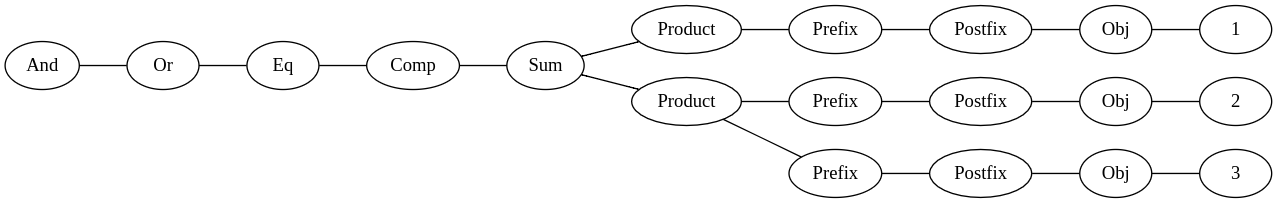
\includegraphics[scale=0.3]{app2assets/tallgraph}
    \end{center}
\end{figure}

\begin{figure}
    \caption{Compressed tree for ``1 + 2 * 3''}
    \label{setanta:compressedtree}
    \begin{center}
    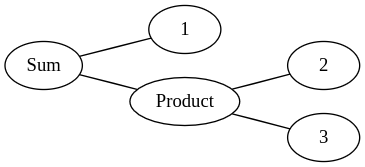
\includegraphics[scale=0.8]{app2assets/smallgraph}
    \end{center}
\end{figure}

\subsection{Async / await slowness}
\label{solution:asyncawaitslowness}

As mentioned in the \hyperref[background:asyncawait]{technical background}, recent versions of JavaScript have introduced a new syntactic construct known as async/await. This feature is intended to get around the problem of writing blocking and asynchronous code in JavaScript. In theory, async / await is just syntactic sugar for the \hyperref[background:asyncawait]{Promises API}, and is recommended to use to improve readability and maintainability of code.

When writing the interpreter for \Setanta{} to allow blocking operations, I took advantage of this new async / await feature, and it did lead to simple easy to read code. However, when I timed my tests, I found that the interpreter had been reduced to running at an absolute crawl. My test suite now took over 13 seconds to execute all programs.

As an experiment, I re-wrote the whole interpreter directly with the Promises API, manually resolving the async / await syntactic sugar, and then I executed my tests again. The results were shocking, the execution time for my tests was reduced down to almost 1 second, a ~13x speedup!

This was highly shocking to me, as I had never heard anything about async / await being slower than the raw Promises API before, in fact, a cursory Google search will bring up countless results of people talking about how the speed of async / await is comparable or even faster than Promises.

\section{The learning environment - \trys{}}

\subsection{High Level Design}

\trys{}, like the other components, is written mainly in TypeScript. The website is built on Google's LitElement library. LitElement is a library to write custom re-usable web components, it's a descendant of the Polymer framework, which has since been deprecated. LitElement is used to achieve a Material Design aesthetic. The text editor component uses the open-source library CodeMirror.

The backend for \trys{} is written in Go and runs on the Google App Engine (GAE) cloud infrastructure platform. The backend for the site supports the ability to save and retrieve \Setanta{} programs to the cloud.

A high-level architecture outline for \trys{} can be seen in Figure~\ref{trysetantadiagram}

\begin{figure}
    \caption{\trys{} High Level Design}
    \label{trysetantadiagram}
    \begin{center}
    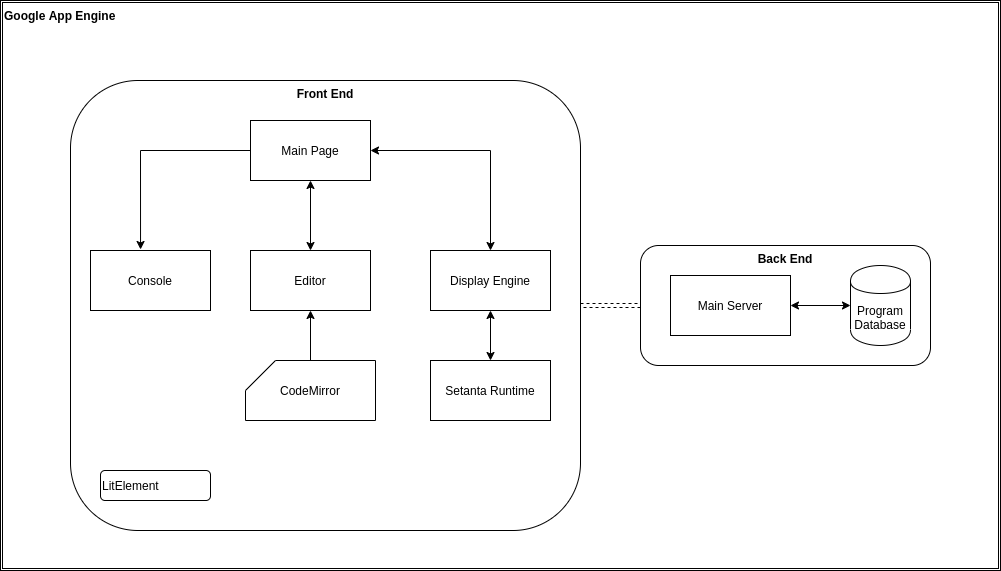
\includegraphics[scale=0.4]{trysetantadiagram}
    \end{center}
\end{figure}

\trys{} is known to work with the Google Chrome, Mozilla Firefox, Safari and Microsoft Edge browsers, however, it does not work with Internet Explorer. This is due to Internet Explorer not supporting the Promises API directly. It should be possible to compile the code down to an earlier version of JavaScript that would work with IE, but this is of very low priority.

\subsection{Graphics API}

To better enable the educational experience on \trys{}, the \Setanta{} runtime has access to a graphics API. The graphics API allows the user to draw simple graphics primitives and animations. This API is exposed to the \Setanta{} program as a global object. The user can access various fields and methods on this object to draw and manipulate shapes on the display. Appendix~\ref{appendix:screenshots} contains screenshots of programs rendering the Sierpinski triangle, and a game of snake (Figure~\ref{screenshot:sierpinski-mobile}, Figure~\ref{screenshot:snake-desktop} respectively).

The graphics API also exposes methods to consume keyboard inputs, so the user can program simple games like \emph{Snake} with ease. It also features a full-screen mode. You can find the \emph{Snake} game demo at \url{https://try-setanta.ie/EhEKBlNjcmlwdBCAgICgxt6JCg}.

\subsection{Saving Code}

\trys{} supports the ability to save a program to a specific URL. Clicking ``Faigh nasc'' (meaning ``get link'') redirects the user to a unique URL with which they can access their code. For example, the Sierpinski triangle example is available at:
\begin{quote}
    \href{https://try-setanta.ie/EhEKBlNjcmlwdBCAgIDgycODCg}{try-setanta.ie/EhEKBlNjcmlwdBCAgIDgycODCg.}
\end{quote}

This feature is handled by the Go backend on the Google App Engine. The programs are stored on the cloud Datastore, each program is identified by a unique integer. This unique integer is encoded into a string key, and this key is the URL where the code can be retrieved.

\subsection{UI/UX Design}

The UI/UX design for the \trys{} website follows the Material Design\cite{material-design} design philosophy. When \trys{} is loaded, you are first brought to a simple landing page that directs the user to either visit the documentation, or open the editor, in English and in Irish.

The learning environment site consists of 3 main components: A console, a graphics canvas and a text editor. They are distributed according the material design method, placed on individual card like components. Contextually relevant actions such as "run code", "stop code" etc are displayed in floating action buttons. Care has been taken to ensure that only the correct buttons are displayed to the user (e.g.\ Only show the run button when code is not running, then switch to a stop button while it is running).

The positioning and layout of the buttons has been chosen to provide implicit context to their functionality. For example: The button to "Run in fullscreen mode" is not displayed by default, but when the user hovers over the "run" button, the run in fullscreen mode button appears above it. This tells the user that the fullscreen mode is an alternative to the usual method of running the code, without explaining it in words.

\textbf{Screenshots of \trys{} are included in Appendix~\ref{appendix:screenshots}.}
